% Conclusion => 1. framework 2 in chapter ? show ? 3. 
% Point to highlight => 1. data flow to communication 2. Arrow abstraction on top of session typed language => 1. compilation to efficient code 2. provided an abstraction of parallel structure

% Future work
% anything => 

% Evaluation => 
% 1. show to code => show 
% 2. show in haskell code
% 3. show the function to generate the code (explain the function)
% 4. how user need complete the definition
% 5. how to compile it and run it
% 2. pick a generated code (put everything in the appendix if you want)
% 6. haskell merge sort v.s merge sort in arrow (highlight the difference => friendly user interface in haskell adapting existing haskell code to adapt it the framework)
% 3. the collection of local type that we derived
\chapter{Parallel algorithms and evaluation} \label{eval} \label{chap:eval}
In this section, we will give an overview of how to use SPar for parallel algorithms, benchmarking the performance of the generated code for various computations and analyzing the design choices of the project.
\section{Parallel algorithms}
The biggest advantage of writing parallel programs in SArrow is that the user can express the computation similar to the sequential one without worrying about any low-level primitives for parallel computations. We will give a recommended recipe of expressing computations in SArrow and a concrete example for the explanation.

\subsection{Four steps to write parallel algorithms in SPar}
Usually, divide-and-conquer algorithms are the best candidates for SPar to parallelize. The recipe is below:
\begin{enumerate}
    \item Understand the algorithm: We recommend programmers to express the algorithms in the recursion schemes (see \secref{b:rs}) Recursion schemes is recommended because it separates the split function, the merge function and the structure of divide-and-conquer from each others so it helps you familiar with the building blocks of the divide-and-conquer algorithms, i.e, the data structures involved, the type signature of the split function, the type signature of merge functions and their implementations.
    \item Systematic parallelization: In the first iteration, we can express the split, merge functions and other necessary helper functions in terms of the SArrow by combing \hask{arr} constructor and \hask{Prim} constructor. Every computation wrapped by \hask{arr} with \hask{Prim} is consider to be sequential. We will substitute them into high-level parallel patterns provided by SPar. For example, divide-and-conquer algorithms can be parallelized by \hask{divConquer} (see \coref{SArrow:dq}) helper functions. Notice that the number determining the level of a parallelized divide-and-conquer algorithm should be set accordingly by the number of cores of the execution machine.
    \item Specific parallelization: The above step is generic and can be applied to any divide-and-conquer algorithm. In this stage, what will be done is determined by the specific implementations. Programmer should inspect the implementation of these function wrapped by \hask{arr} with \hask{Prim} to see whether there are any parallelism to exploit. If so, programmer should rewrite these functions by the parallel patterns provided by SPar or arrow combinators. For example, the split function of the Quickhull \cite{Quickhull2019} to solve convex hull problems will use a for-loop to find the point whose distance to the line is at the maximum. This step can be expressed by the parallel map-and-reduce pattern (see \coref{arrow:code:preduc}). Programmers can apply this step iteratively until all possible parallelisms are exploited or programmers think it is enough. All the sequential computation are left in the form: \hask{arr} with \hask{Prim}.
    \item Wrap up: Before the code generation, programmer need to implement all the \hask{Prim} functions in terms of the target language. In the scope of this project, programmer will write them in C and create a header file. The generated code will include the header file and from then on, programmers obtain the parallelized version of the algorithm that is guaranteed to be deadlock-free.
\end{enumerate}
\subsection{Example: Merge sort}

We will show how to use the framework to generate parallel code by expressing merge sort on a list of integer.
\begin{enumerate}
\begin{listing}[ht]
\begin{minted}{Haskell}
split :: SArrow [Int] (Either (Either () Int) ([Int], [Int]))
split = arr $ Prim "split" undefined
    
merge :: SArrow (Either (Either () Int) ([Int], [Int])) [Int]
merge = arr $ Prim "merge" undefined
    
sort :: SArrow [Int] [Int]
sort = arr $ Prim "sort" undefined
\end{minted}
\caption{The code for atomic functions}
\label{eval:code:step1}
\end{listing}
    \item The first step is to understand algorithms. The merge sort is a quite famous divide-and-conquer algorithm. It splits the list into two halves, apply the algorithm to sub-lists recursively and finally merge the sub-lists by an order. From the above description, we identify three atomic functions \hask{split}, \hask{merge} and the base function \hask{sort}.  We need to define the type signatures for these functions to understand what data structures are involved. For the \hask{split} function, it will take a list of integers \hask{[Int]} as an input and output a pair of lists of integers \hask{(Int, Int)} as an output. To deal with the case where the input list can not be split i.e when the list is empty or a singleton list, we wrap the output pair with a either type to deal with these situations. So the output type is \hask{Either (Either () Int) ([Int], [Int])} Accordingly, the type signature of \hask{merge} is the reverse of the \hask{split}. \hask{sort} type signature will be the same as the merge sort: \hask{[Int] -> [Int]}. Finally, we wrap them using Prim and arr. The code written for the first step is shown in the \coref{eval:code:step1}.
\begin{listing}[ht]
\inputminted{Haskell}{eval/step2.hs}
\caption{Construction of the algorithm using the parallel pattern and atomic functions}
\label{eval:code:step2}
\end{listing}
    \item The second step is combine these atomic function in the first step in a parallel pattern we define. Since we are using our framework to parallelizing a merge sort, we will use the divide-and-conquer parallel pattern. The result of applying the pattern pattern is an expression whose type is \hask{Int -> SArrow [Int] [Int]} where the first parameter determines the number of level of the divide-and-conquer algorithm. In this case, we will use our refined version of divided-and-conquer parallel pattern that support shortcut. The code written for the second step is shown \coref{eval:code:step2}. For the completeness, we also include the implementation of the parallel pattern. The polymorphic parallel pattern can be used to generate non-polymorphic code. 
    \item The third step is optimizing the atomic function. Since split and merge are not very intensive computation. We will not modify anything for this step.
\begin{table}[ht]
\begin{subtable}{\textwidth}
\inputminted{C}{eval/data.h}
\caption{data.h}
\end{subtable}
\vskip\baselineskip
\begin{subtable}{\textwidth}
    \inputminted{C}{eval/func.h}
    \caption{func.h}
\end{subtable}
\vskip\baselineskip
\begin{subtable}{\textwidth}
    \inputminted{C}{eval/code.c}
    \caption{code.c}
\end{subtable}
\caption{The complete structure of the generated c code. Omit the  implementation of code.c} 
\label{eval:code:step4}
\end{table}
    \item Up to this step, we have finished everything we need to do in the Haskell side to express computation. First of all, we will show how to generate C code from a SArrow expression using the framework. Secondly, we will talk about how to complete the implementation for the atomic functions. In the library, we have defined a function \hask{codeGen} that takes an SArrow expression as an input and generates three files in the specified path. The first file is called func.h which contains declarations of all atomic functions. The second file is data.h which includes the definition of data structures involved in C. The third file is code.c which includes all the necessary headers like standard library and channel library and generated code. The structure is similar to what we described in \secref{codegen:sec:structure}. The last job to do is to complete the implementation of the functions declared in the func.h. After that, we use the generated code in whatever way we want. The structures are shown in \tabref{eval:code:step4}.
\end{enumerate}
\begin{listing}[ht]
    \begin{minted}{text}
0: !<1, [Int]>.?(4, [Int]).end
1: ?(0,[Int]).Br<[2,3,4],
    {L: !<4,Either (Either () Int) ([Int],[Int])>.end, 
     R: !<3,([Int],[Int])>.Br<[2],
        {L: !<2,Either (Either () Int) ([Int],[Int])>.end, 
        R: !<2,([Int],[Int])>.!<2,[Int]>.end}>
        .end}>
    .end
2: &(1,
    {L: end, 
    R: &(1,
        {L: ?(1,Either (Either () Int) ([Int],[Int])).end,
        R: ?(1,([Int],[Int])).?(1,[Int]).end}).!<4,[Int]>
        .end})
    .end
3: &(1,{
    L: end, 
    R: ?(1,([Int],[Int])).Br<[4],
        {L: !<4,Either (Either () Int) ([Int],[Int])>.end,
        R: !<4,([Int],[Int])>.!<4,[Int]>.end}>
        .end})
    .end
4: &(1,
    {L: ?(1,Either (Either () Int) ([Int],[Int])).end, 
    R: &(3,
        {L: ?(3,Either (Either () Int) ([Int],[Int])).end,
        R: ?(3,([Int],[Int])).?(3,[Int]).end})
        .?(2,[Int]).end})
    .!<0,[Int]>.end
    \end{minted}
    \caption{Inferred session types} 
    \label{eval:code:stypes}
\end{listing}

In addition to the generated code, we also show the inferred session types of each role in the system for the merge sort at level two in \coref{eval:code:stypes}. We can simply call the function \hask{runType} on any SArrow expression to get a list of session types. The session types is pretty printed. The original representation of session types is in free-monad as explained in \charef{chap:spar}. \hask{br} is a syntax sugar for a series of select (see in \secref{spar:sec:session-typing}).

\section{Benchmarks}
\begin{listing}[ht]
\begin{minted}{C}
int main()
{
    int * tmp = randomList(1048576);
    List_int a = (List_int) {1048576, tmp};
    double start = get_time();
    proc0(a);
    double end = get_time();
    printf("%lf\n", end - start);
    return 0;
}
\end{minted}
    \caption{The main function for benchmark}
    \label{eval:code:main}
\end{listing}
We have defined a specific code generation function for benchmarking the parallel algorithms. The main difference from the normal generated code is the main function. The main function will create a random source data by the specified input size, record the execution time and output the execution time. The main file is shown in \coref{eval:code:main}. 

For each benchmark of a divide-and-conquer SArrow, we will generate the code for a range of size and for different number of unroll representing the level of the algorithms. We will record the execution time on normal laptop as well as high performance computer.

The compiler we used is gcc (version 9.1.0) with the default optimization. The two platform we run our benchmark on 1) Intel i5-8259u with 4 physical core 2) 32 cores high throughput computing machine provided by Imperial College London ICT services \footnote{http://www.imperial.ac.uk/admin-services/ict/self-service/research-support/rcs/computing/high-throughput-computing/}.

We have implemented three benchmark to run.
\begin{enumerate}
    \item \textbf{Merge sort. } It is one of the most classic divide-and-conquer algorithms. Its details are shown in the above subsection.
    \item \textbf{Dot product. } It computes the inner product of two vectors whose sizes are the same and of the form $2^n$.
    \item \textbf{Int count. } It counts the number of occurrence of integer given a list of integer ranging from 0 to 50. \hask{split} divides the list by halves. \hask{count} will count the occurrence of integers and output a list of tuple where the integer is the value and the second integer is the number of occurrence of that value. \hask{union} will union the resulting of sub-lists by summing up the occurrence.
\end{enumerate}
\subsection{Evaluation}
We will demonstrate the execution time against different sizes for different levels of divide-and-conquer algorithms as well as the speedup of the parallel algorithms against the sequential algorithm.
\begin{figure*}[ht]
    \begin{subfigure}[b]{0.475\textwidth}
        \centering
        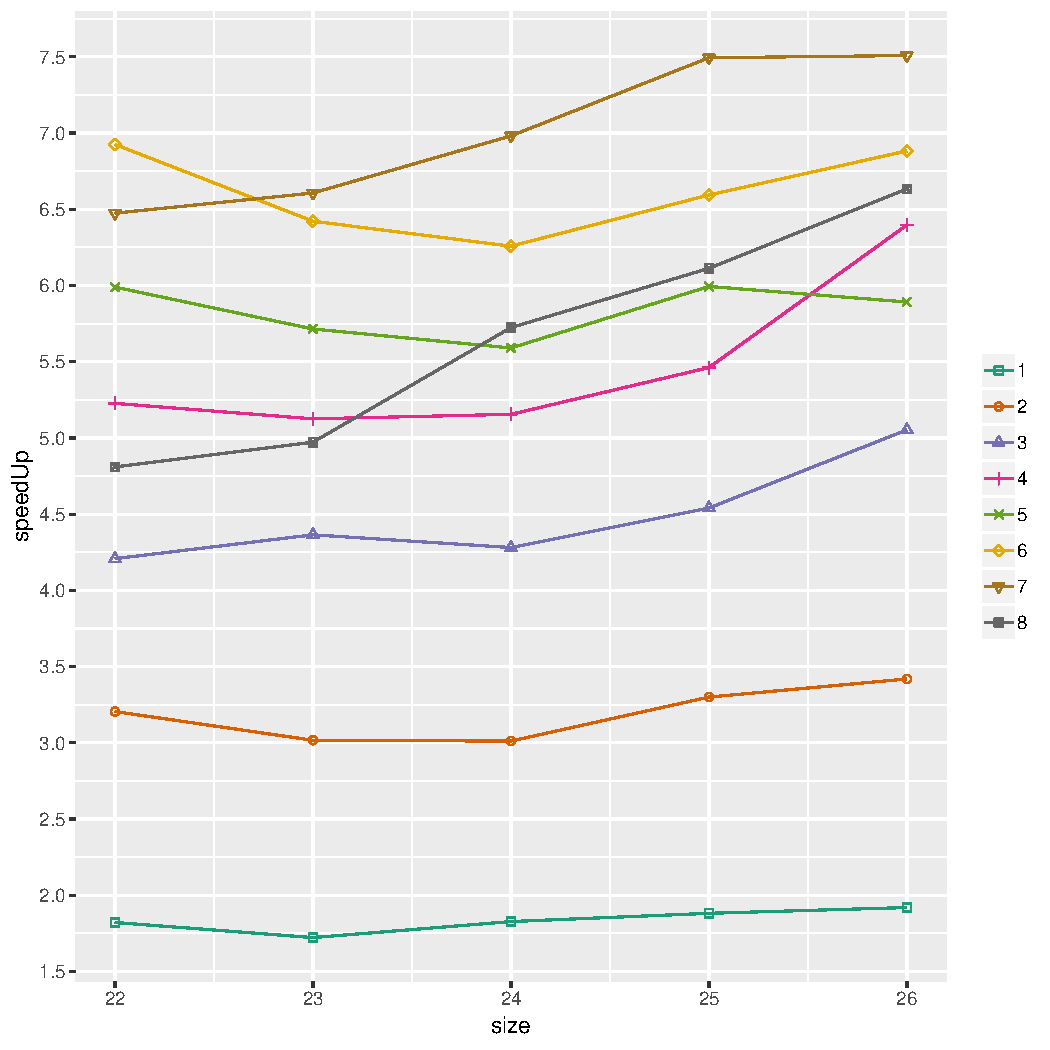
\includegraphics[width=\textwidth]{eval/mergesort-speedup.pdf}
        \caption{Merge sort: speedup}
        \label{eval:fig:ms:speed}
    \end{subfigure}
    \hfill
    \begin{subfigure}[b]{0.475\textwidth}
        \centering
        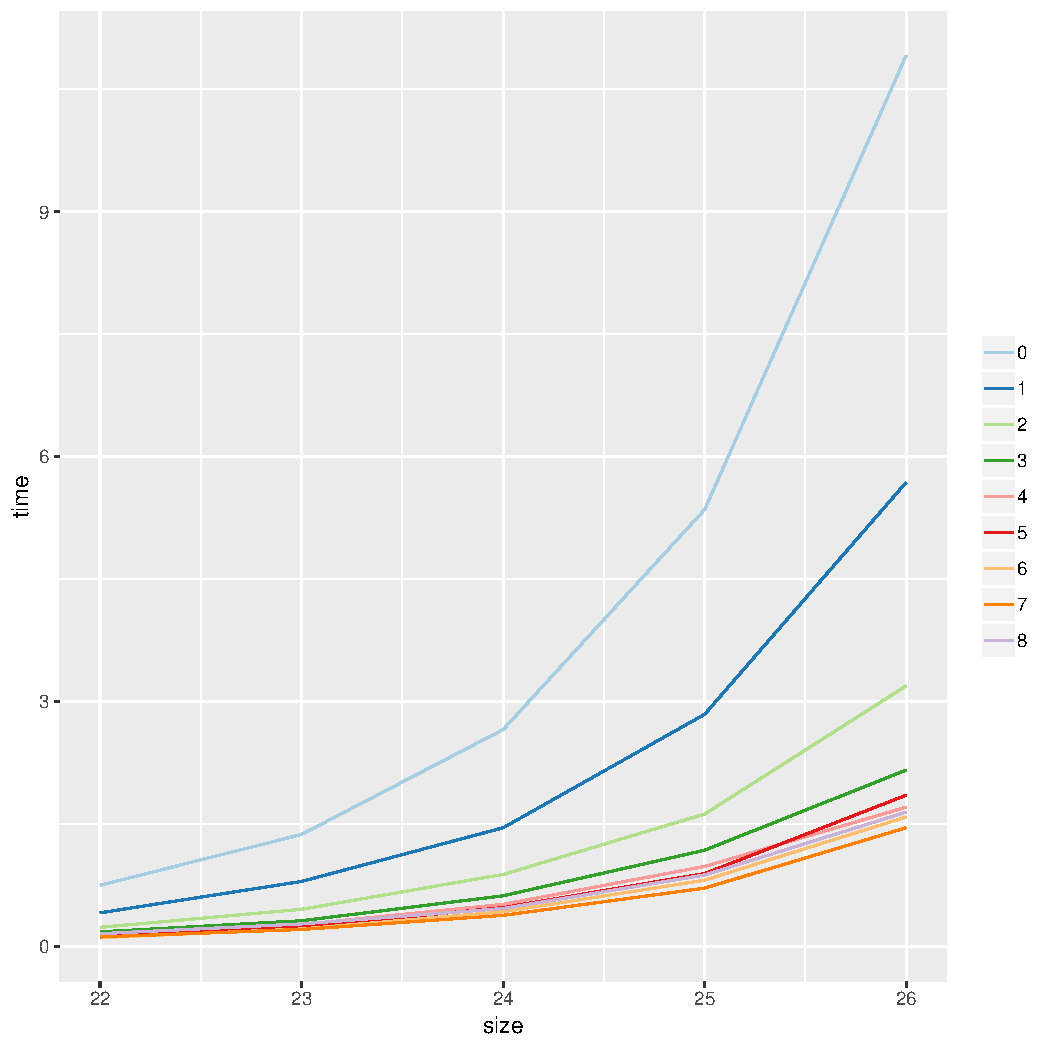
\includegraphics[width=\textwidth]{eval/mergesort-time.pdf}
        \caption{Merge sort: execution time}
    \end{subfigure}
    \vskip\baselineskip
    \begin{subfigure}[b]{0.475\textwidth}
        \centering
        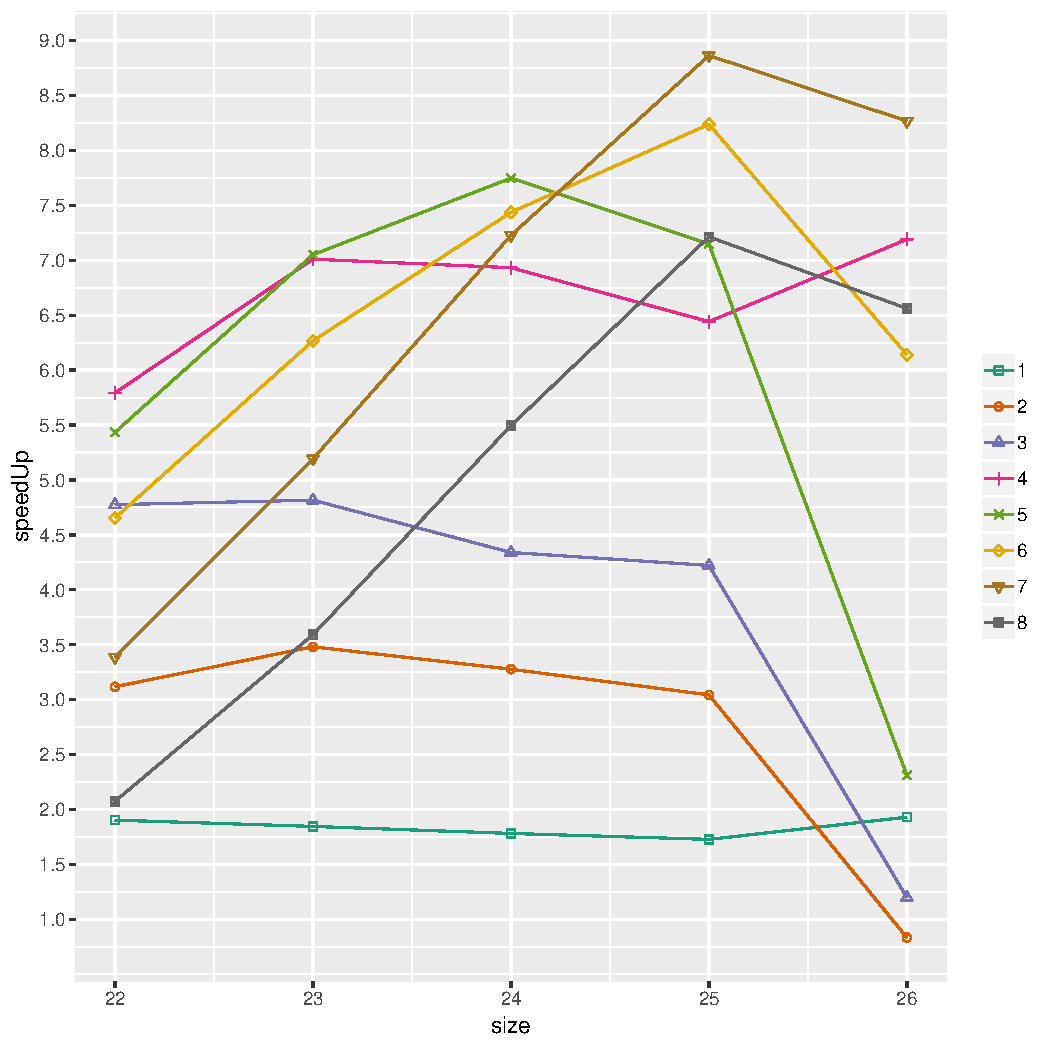
\includegraphics[width=\textwidth]{eval/dotprod-speedup.pdf}
        \caption{Dot product: speedup}
    \end{subfigure}
    \hfill
    \begin{subfigure}[b]{0.475\textwidth}
        \centering
        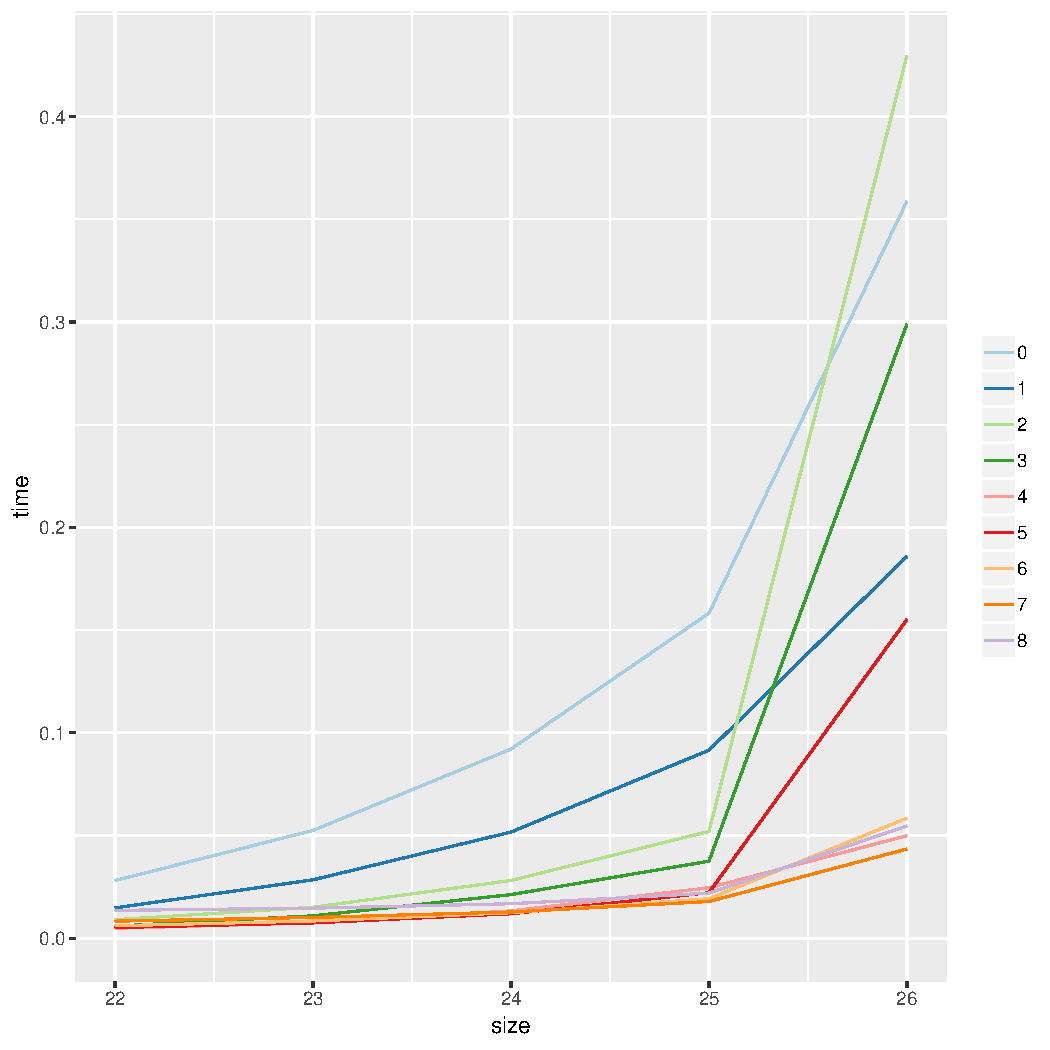
\includegraphics[width=\textwidth]{eval/dotprod-time.pdf}
        \caption{Dot product: execution time}
    \end{subfigure}
    \vskip\baselineskip
    \begin{subfigure}[b]{0.475\textwidth}
        \centering
        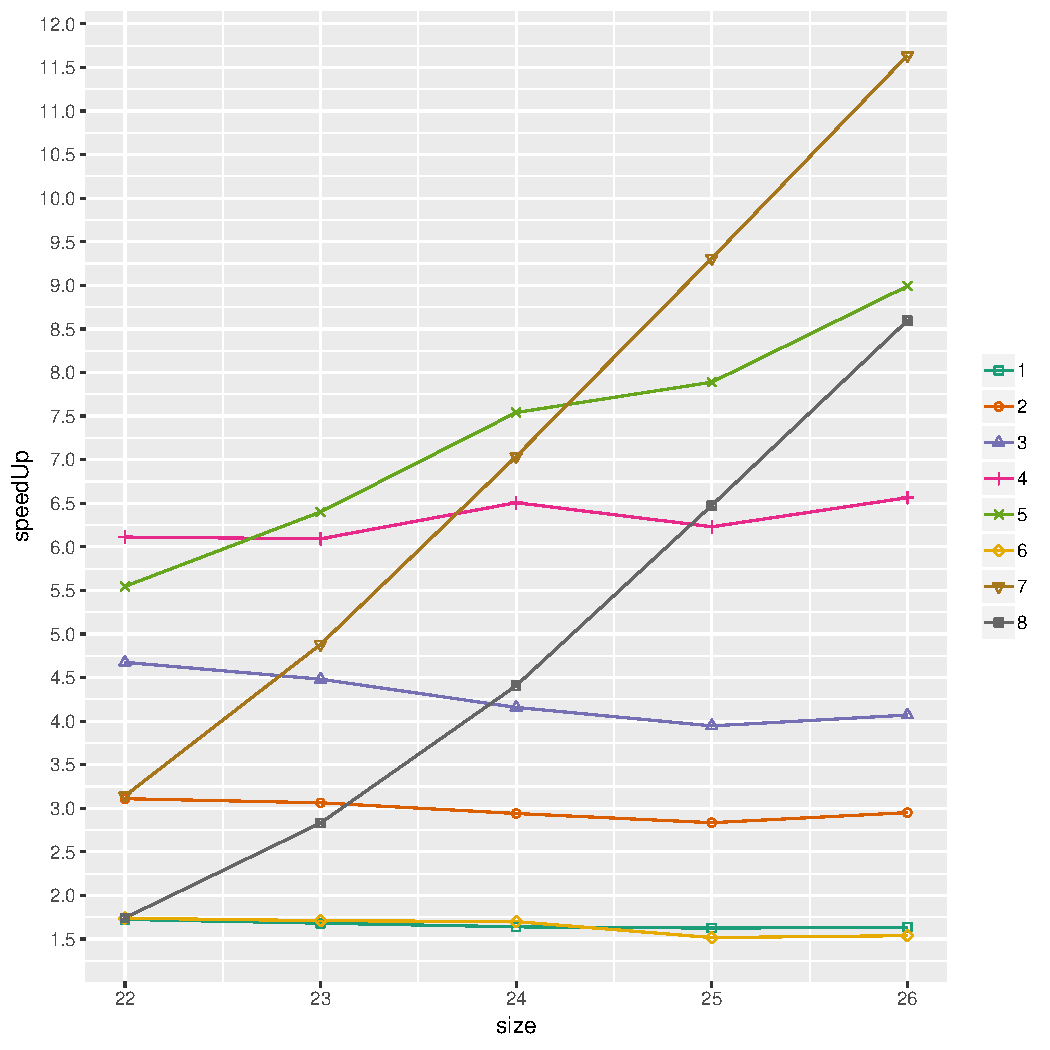
\includegraphics[width=\textwidth]{eval/intcount-speedup.pdf}
        \caption{Int count: speedup}
    \end{subfigure}
    \hfill
    \begin{subfigure}[b]{0.475\textwidth}
        \centering
        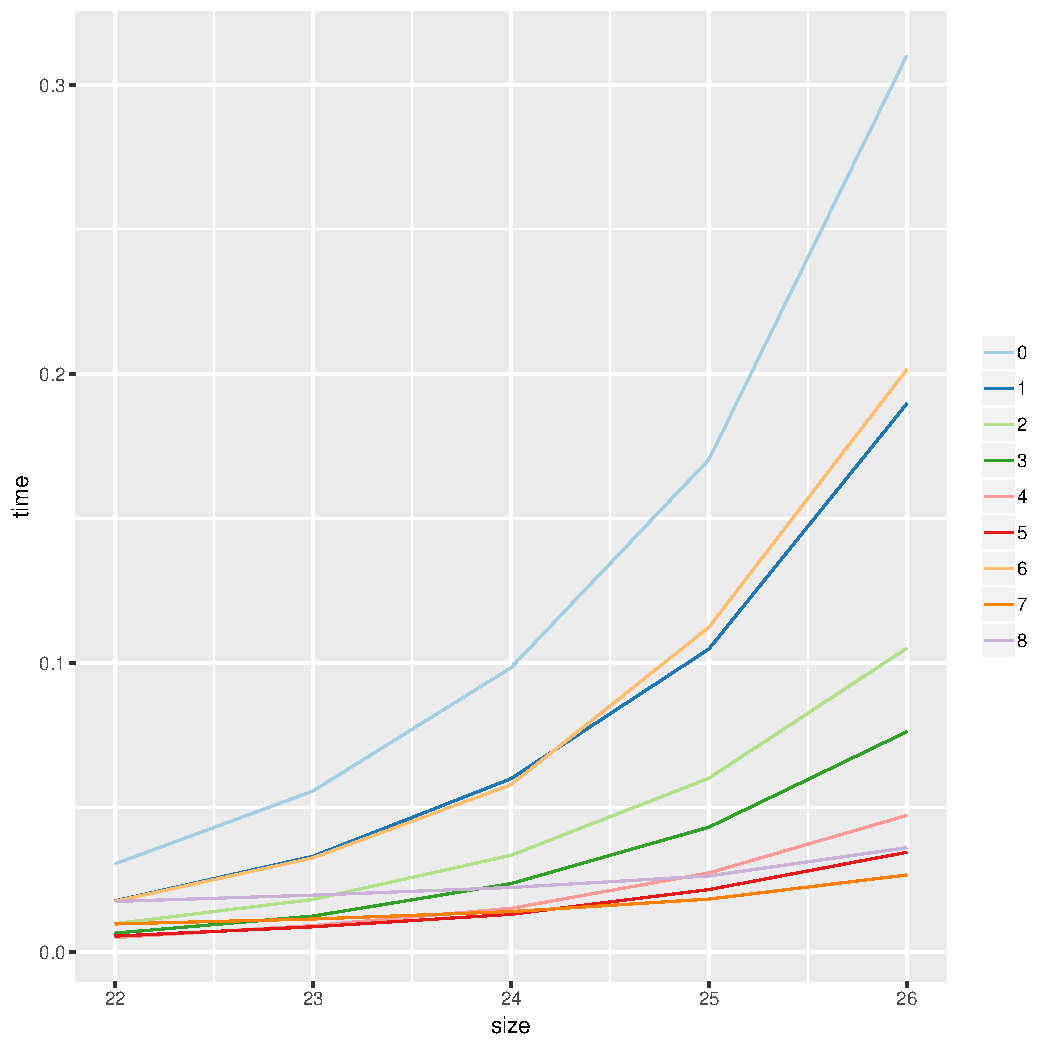
\includegraphics[width=\textwidth]{eval/intcount-time.pdf}
        \caption{Int count: execution time}
    \end{subfigure}
    \caption{Benchmarks results}
    \label{eval:fig:finalresult}
\end{figure*}
\figref{eval:fig:finalresult} shows the result for different cases running on a 32-core machine. For each level $k$, we will generate a total number of $2^k$ threads to execute the parallel computation. The x axis indicates the size of the input where 22 means the input is a list of $2^20$ integers or a pair of list of $2^20$ integers. The execution time is measured in seconds and the speedup is computed by $\frac{t_{\text{sequential}}}{t_\text{parallel}}$. 

For merge sort, the speedup increases as the size increases which is shown by the increasing graph from \figref{eval:fig:ms:speed}. It is valid for all the level due to all the lines are increasing. Different levels will have different degree of performance boost on increasing sizes. For dot product, this trend holds for up to size 26. When the size is 26, we witness a sudden decrease in speedup at various levels. The reason for this abnormal behavior is yet to be studied. As for the int count, the speedup increases against increasing sizes when the level is big enough. The degree of speedup increase at the large level is also the most obvious for int count among the three benchmark. This can be observed by the two slope when level = 7 and level = 8. Unexpected behavior is the line when level = 6. Its speedup is nearly as small as level = 1. Also, overproduction of threads has positive impacts on the speedup. The best level is 7 which contains 128 threads. It gives a 7.5X speedup for merge sort, 8X speedup for dot product and nearly 12X speed up for int count when the size is $2^{26}$. In general, greater number of threads has better speedup for greater sizes. The level that gives the best performance depends on the number of cores of the machine. The relationship is not simply one-to-one and from experiment, we recommend to overproduce the number of threads compared the number of cores. However, the performance will not be increased greatly and even slower if the level is too big (see the comparison of speedup line for level = 7 and 8).